%--------------------------------------------%
%--------------------------------------------%
%    PROPOSED SOLUTION 
%--------------------------------------------%
%--------------------------------------------%

\section{Proposed solution}

\subsection{Overview}

% FRAME: OVERVIEW OF PROPOSED SOLUTION
\begin{frame}{Proposed solution: overview}
\begin{figure}[hbt!]
  \centering
  \includegraphics[width=0.8\columnwidth]{{{diagram_proposed_solutions}}}
  %\caption{[1] A. N. L. Fred and A. K. Jain, “Combining multiple clusterings using evidence accumulation,” IEEE Transactions on Pattern Analysis and Machine Intelligence, vol. 27}
  \label{fig:eac kmin evo}
\end{figure}

\end{frame}

\begin{frame}{Proposed solution: final}
\begin{figure}[hbt!]
  \centering
  \includegraphics[width=1.0\columnwidth]{{{diagram_proposed_solutions_BAD}}}
  %\caption{[1] A. N. L. Fred and A. K. Jain, “Combining multiple clusterings using evidence accumulation,” IEEE Transactions on Pattern Analysis and Machine Intelligence, vol. 27}
  \label{fig:eac kmin evo}
\end{figure}

\end{frame}

%--------------------------------------------%
%    PRODUCTION PHASE
%--------------------------------------------%
\subsection{Production}

\begin{frame}{Optimizing production of ensemble}

\begin{itemize}

\item K-Means is simple and has been used with EAC before with success.

\item K-Means:

  \begin{itemize}
  \item \textbf{labelling}: find the closest centroid to each data pattern
  % $$
  % l_i = arg \: \min_k \;d(x_i, c_k)
  % $$
  \item \textbf{update}: new centroids are the mean of the assigned patterns
  % $$
  % c_k = \sum_{i : l_i = k} x_i
  % $$

  \end{itemize}

\item Number of clusters from interval [$K_{min},K_{max}$]

\item Optimization through parallelization in GPU.

\end{itemize}

\end{frame}



\begin{frame}{GPGPU K-Means}

\begin{itemize}

\item CUDA GPGPU

  \begin{itemize}
  \item Hundreds of processors

  \item \emph{Single instruction multiple thread} approach

  \item Shared memory between threads

  \end{itemize}
\end{itemize}

\end{frame}



\begin{frame}{GPU K-Means}

\begin{itemize}

% \item CUDA GPGPU
\item GPU

  \begin{itemize}
  \item Hundreds of processors

  \item \emph{Single instruction multiple thread} approach

  \item Shared memory between threads

  \end{itemize}

\item Parallel K-Means

  \begin{enumerate}

  \item Host sends data and centroids to GPU

  \item GPU threads compute the closest centroid to data patterns.

  \item The label and distance are stored and transfered to host.

  \item Host computes new centroids and sends them back to host.

  \item Repeat steps 2-4 until stopping criteria is met.

  \end{enumerate}

\end{itemize}

\end{frame}



        
%--------------------------------------------%
%    COMBINATION PHASE
%--------------------------------------------%
\subsection{Combination}

\begin{frame}{Optimizing combination}

\begin{itemize}

\item Biggest challenge: $O(n^2)$ memory complexity
  \begin{itemize}
  \item $200\:000$ dataset $\longrightarrow$ $149$ GB
  \item $1\:000\:000$ dataset $\longrightarrow$ $3725$ GB
  \end{itemize}

\item Co-association matrix is:
  \begin{itemize}
  \item symmetric ($49.5\%$ reduction)
  \item sparse (association density as low as $1\%$)
  \end{itemize}

\item \textbf{exploiting sparsity}

% \item Two approaches:
%   \begin{itemize}
%   \item using prototypes
%   \item \textbf{exploiting sparsity}
%   \end{itemize}

\end{itemize}

\begin{center}
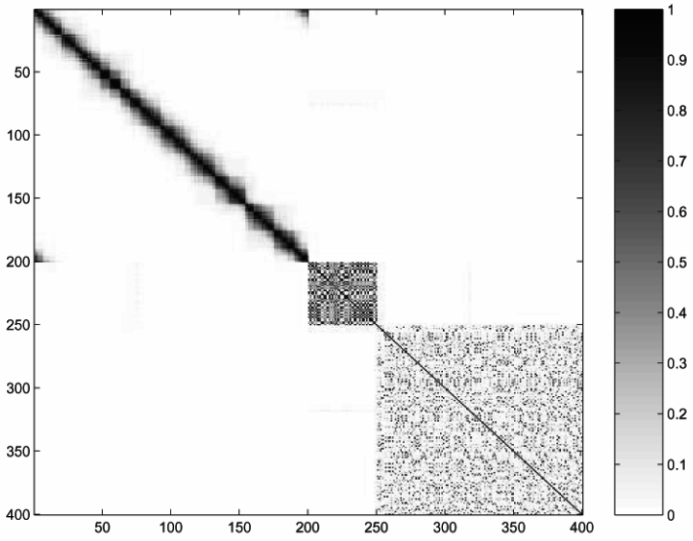
\includegraphics[width=0.3\textwidth]{EAC_plots/coassocEAC}
\end{center}

\end{frame}



\begin{frame}{Optimizing combination}

\begin{itemize}

%\item Sparse formats: LIL, DOK, COO, CSR, CSC

\item Library solutions are either very slow or occupy too much memory

\item Lack of literature on fast building

\item Compromise between speed and memory: \\
\centering
\Large{\textbf{EAC CSR}}

  % \begin{itemize}
  % \item \Large{\textbf{EAC CSR}}
  % \end{itemize}

\end{itemize}

\end{frame}


% plot for coming up with assumption for number of associations
% \begin{frame}{Optimizing combination}
% \begin{center}
%   \includegraphics[width=0.8\columnwidth]{{{max_assoc_bgs}}}
% \end{center}
% \end{frame}


\begin{frame}{Optimizing combination}
\begin{center}
  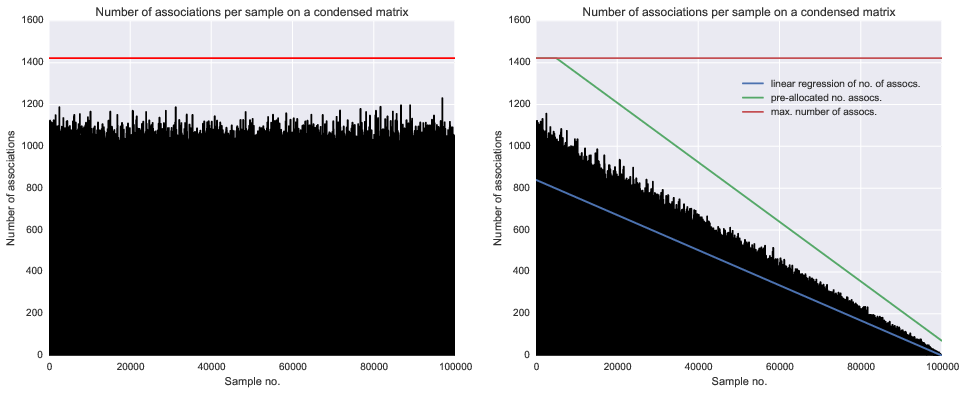
\includegraphics[width=0.8\columnwidth]{eac_csr_cond_full_degree_100k.png}
\end{center}
\end{frame}


%--------------------------------------------%
%    RECOVERY PHASE
%--------------------------------------------%
\subsection{Recovery}

\begin{frame}{Optimizing final clustering}

\begin{itemize}

\item Single-Link (SL) has been used before with success

\item SL is a hierarchical agglomerative algorithm

\item SL works on a pair-wise proximity matrix between all patterns

\item SL is equivalent to a Minimum Spanning Tree (MST)

\item Disk based MST variant to address very large co-association matrices

\end{itemize}

% used MST based Single-Link to process only real associations.
% Used out-of-core sorting algorithm from PyTables for sorting the associations.
\end{frame}